% s_applications.tex -- final report: where the result matters in practice, and what to study next.
% Figure figs/appmap.pdf is made by fpga/host/plot_report_extras.py (illustrative calculation, see the caption).
% Written with AI assistance (Claude, Anthropic), project decision D-06.

\section{Real-World Relevance and Future Research}
\label{sec:applications}
\nb{Every adaptive equalizer in a moving or drifting environment faces the question this project measured: how fast may the channel change before the filter can no longer follow it? This section places the measured limit next to real links, lists where the hardware result is useful, and sets out the research it opens.}

\subsection{Where real channels sit relative to the measured limit}
\label{sec:appmap}
\nb{The variation rate $S$ is a laboratory analogue of the normalised Doppler $f_DT_s$ (\cref{sec:intro}). Taking one full period of the primary triangle trajectory, $152S$ symbols, as one fading cycle gives $\nu=1/(152S)$ cycles per symbol, and the \lvl{L1} boundaries $S^\star_{\rm MSE}=112$, 28 and 10 (primary channel, 16\,dB, \cref{tab:sstar}) become $\nu^\star\approx5.9\times10^{-5}$, $2.3\times10^{-4}$ and $6.6\times10^{-4}$ for $\mu=2^{-10}$, $2^{-8}$ and $2^{-6}$. For a real link $f_D=vf_c/c$ and $\nu=f_D/R_s$. \Cref{fig:appmap} places typical single-carrier links on the same axis \cite{jakes1974,proakis2008}:}
\begin{itemize}\itemsep0pt
\item \nb{\emph{HF skywave modems} (Doppler spread 0.1--1\,Hz at 2400\,Bd) are within reach of $\mu=2^{-6}$, and of $\mu=2^{-8}$ for Doppler spreads up to about 0.5\,Hz.}
\item \nb{\emph{A vehicular link} at 2\,GHz and 1\,Msymbol/s sits just inside the $\mu=2^{-8}$ limit at highway speed, while $\mu=2^{-10}$ would already lose accuracy at about 30\,km/h: the step size is a speed rating.}
\item \nb{\emph{Single-carrier cellular} at 900\,MHz and 270.8\,ksymbol/s is trivial for pedestrians but passes even the $\mu=2^{-6}$ limit near 210\,km/h; \emph{high-speed rail} at 200--350\,km/h lies entirely beyond it.}
\item \nb{\emph{Underwater acoustic links} combine slow sound with low symbol rates and reach $\nu\sim10^{-2}$, far beyond plain LMS; this agrees with the literature, where coherent underwater receivers pair adaptive equalization with carrier tracking and faster adaptation \cite{stojanovic1994}.}
\end{itemize}
\nb{\emph{What the map does not claim.} The triangle trajectory is deterministic and sweeps one tap, whereas real fading is random and moves all taps; the channel is three taps long and the noise level is fixed. The map is therefore an order-of-magnitude comparison that tells which regime a link is in --- comfortably trackable, near the limit, or beyond plain LMS --- not a prediction of exact speeds. Testing it with a random-fading channel is the first item of \cref{sec:future}.}

\begin{figure}[t]
\centering
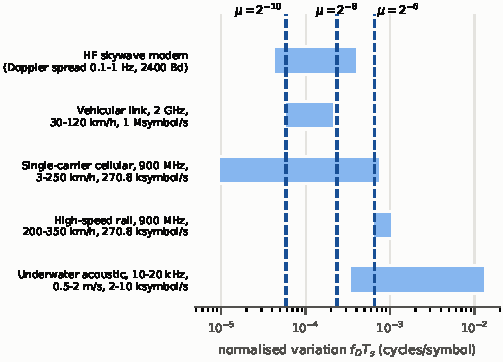
\includegraphics[width=\linewidth]{figs/appmap.pdf}
\caption{\nb{Illustrative map of real channels against the measured tracking limit. Bars: $\nu=f_DT_s$ from the stated carrier, speed and symbol-rate ranges ($f_D=vf_c/c$; textbook values, not measurements). Dashed lines: \lvl{L1} boundaries $S^\star_{\rm MSE}$ (primary channel, 16\,dB) converted with $\nu^\star=1/(152S^\star)$. Order of magnitude only: the experiment uses a deterministic triangle trajectory, not random fading.}}
\label{fig:appmap}
\end{figure}

\subsection{Where the hardware result is useful}
\label{sec:uses}
\begin{itemize}\itemsep0pt
\item \nb{\emph{Choosing the step size from the required speed.} The boundary $S^\star_{\rm MSE}\approx0.11/\mu$ (\cref{sec:p3}) and its first-order explanation (\cref{sec:theory}) turn ``how fast will the platform move'' into ``which power-of-two $\mu$'' --- for vehicular, rail, drone and maritime single-carrier links --- with the measured cost of 51 DSP slices for three parallel 16-tap receivers.}
\item \nb{\emph{Low-cost fixed-point equalizers.} With round-to-nearest updates a 12-bit multiplier word and a 16-bit accumulator track as well as 26 bits, while truncation needs about two more bits (\cref{sec:fxp,sec:board}). Slowly drifting channels --- wireline links, and the adaptive equalizers of coherent optical receivers \cite{savory2010} --- live in this static-misadjustment regime, where the word-length result applies directly.}
\item \nb{\emph{Narrowband links with spare hardware.} At 6.25\,Msymbol/s the design runs 600 to 2600 times faster than HF and underwater symbol rates, so one device could serve many channels by time-multiplexing the same datapath.}
\item \nb{\emph{A reproducible channel emulator.} Because the board reproduces the bit-true model count for count, it is a hardware-in-the-loop test bench: any equalizer placed beside R3 can be compared on the identical impaired stream, with BER and MSE counters and real payloads, at millions of symbols per second.}
\end{itemize}

\subsection{Future research directions}
\label{sec:future}
\begin{enumerate}\itemsep0pt
\item \nb{\emph{Random fading.} Replace the triangle controller by a sum-of-sinusoids Doppler generator in RTL \cite{jakes1974} and measure the boundary directly in $f_DT_s$, which tests the map of \cref{fig:appmap}.}
\item \nb{\emph{Faster adaptation for the high-mobility regime.} NLMS \cite{nagumo1967,slock1993} and RLS \cite{eleftheriou1986} on the same board, reporting tracking gain against hardware cost; 69 of the 120 DSP slices are still free.}
\item \nb{\emph{A step size that follows the channel.} The optimum step grows with the variation rate (\cref{sec:muopt,sec:theory}); a controller that estimates the rate from the error and selects $\mu$ \cite{haykin2014} would remove the fixed speed rating.}
\item \nb{\emph{A realisable receiver.} Decision-directed and pilot-assisted adaptation on the board \cite{mazo1980}, with the payload as data rather than as a known reference.}
\item \nb{\emph{Higher symbol rates.} Beyond the 10-clock update the loop must be pipelined, which turns it into delayed LMS \cite{long1989}; measuring how much tracking that costs is the hardware counterpart of this study.}
\item \nb{\emph{The onset of underflow.} Narrower accumulators (10--14 bits), truncation and step-size approximations \cite{constantinides2003,khan2023} on the board, to find where precision, not $\mu$, sets the boundary.}
\item \nb{\emph{A physical channel and better noise.} An RF or acoustic front end in place of the emulated channel, and a Gaussian noise generator \cite{lee2006} so that hardware BER below $10^{-4}$ can be quoted.}
\item \nb{\emph{Longer and harder channels.} Fractionally spaced and decision-feedback structures \cite{gitlin1982,proakis2008} for non-minimum-phase and longer delay spreads.}
\end{enumerate}
